% ============================================================================
% IEEE Conference Paper: Kubernetes Ingress Load Balancing
% A Quantitative Analysis on Azure AKS
% ============================================================================
\documentclass[conference]{IEEEtran}

% --- Essential Packages ---
\usepackage{cite}
\usepackage{amsmath,amssymb,amsfonts}
\usepackage{algorithmic}
\usepackage{graphicx}
\usepackage{textcomp}
\usepackage{xcolor}
\usepackage{booktabs}
\usepackage{multirow}
\usepackage{hyperref}
\usepackage{listings}
\usepackage{float}
\usepackage{subcaption}
\usepackage{array}
\usepackage{url}

% --- Listings Configuration for YAML and Python ---
\lstdefinelanguage{yaml}{
  keywords={apiVersion, kind, metadata, name, annotations, spec, ingressClassName, rules, http, paths, path, pathType, backend, service, port, number, selector, replicas, matchLabels, template, containers, image, ports, containerPort, resources, requests, limits, cpu, memory, env, value, type},
  sensitive=true,
  comment=[l]{\#},
  morestring=[b]',
  morestring=[b]"
}

\lstset{
  basicstyle=\ttfamily\scriptsize,
  breaklines=true,
  frame=single,
  captionpos=b,
  numbers=left,
  numberstyle=\tiny\color{gray},
  keywordstyle=\color{blue},
  commentstyle=\color{green!50!black},
  stringstyle=\color{red!70!black},
  showstringspaces=false,
  tabsize=2
}

% --- Path to Figures ---
\graphicspath{{Metrics-Graphs_Tables/}}

\def\BibTeX{{\rm B\kern-.05em{\sc i\kern-.025em b}\kern-.08em
    T\kern-.1667em\lower.7ex\hbox{E}\kern-.125emX}}

\begin{document}

% ============================================================================
% TITLE
% ============================================================================
\title{A Comparative Analysis of NGINX Ingress Load Balancing Algorithms on Azure Kubernetes Service Under High-Stress and Fault-Tolerant Conditions}

\author{
\IEEEauthorblockN{Hiten Raj Singh, Aakarsh Jha}
\IEEEauthorblockA{
School of Computer Science and Engineering \\
Manipal Institute of Technology \\
Manipal, India \\
Under the Guidance of: Anjana S.}
}

\maketitle

% ============================================================================
% ABSTRACT
% ============================================================================
\begin{abstract}
As cloud-native microservice deployments grow in scale, the choice of load balancing algorithm at the Ingress layer has a direct impact on application performance and reliability. This paper presents a comparative analysis of three NGINX Ingress Controller load balancing algorithms---Round Robin, Least Connections (via Exponentially Weighted Moving Average), and IP Hashing---deployed on a two-node Azure Kubernetes Service (AKS) cluster. A containerized echo server is subjected to traffic loads of 50, 100, and 200 simulated concurrent users using the Locust framework, with response latency, throughput, CPU resource distribution, and fault tolerance behavior being recorded at each tier. The 200-user tier includes a deliberate pod termination to simulate node failure. Results show that while all three algorithms produce similar average latencies ($\approx$87--90\,ms) and throughput ($\approx$22\,RPS) under baseline conditions, their tail-latency profiles (P99) differ noticeably: Round Robin reaches 170\,ms compared to 110--120\,ms for EWMA and IP Hash. CPU distribution analysis under 100-user load reveals IP Hashing's single-point-of-load problem (CV\,=\,95.5\%) versus Round Robin's even balance (CV\,=\,0.1\%). During fault injection, Round Robin and Least Connections show recovery spikes of $\approx$5111\,ms, while IP Hashing recovers in 504\,ms due to its sticky routing behavior. These findings offer practical guidelines for selecting load balancing strategies suited to specific Kubernetes workload requirements.
\end{abstract}

% ============================================================================
% KEYWORDS
% ============================================================================
\begin{IEEEkeywords}
Load Balancing, Kubernetes, Azure AKS, NGINX Ingress Controller, Round Robin, EWMA, IP Hashing, Fault Tolerance, Cloud Computing
\end{IEEEkeywords}

% ============================================================================
% I. INTRODUCTION
% ============================================================================
\section{Introduction}

Container orchestration platforms, particularly Kubernetes, have changed how distributed applications are deployed and managed in cloud environments \cite{burns2016borg}. As microservice architectures scale to handle large volumes of requests, the load balancing layer---responsible for distributing incoming traffic across backend pods---plays a major role in determining application performance, reliability, and user experience \cite{gandhi2014autoscale}.

Kubernetes provides several abstractions for traffic management, including Services, Ingress resources, and external load balancers. The NGINX Ingress Controller, one of the most widely deployed Ingress implementations, supports multiple upstream load balancing algorithms that can be configured via simple annotation-based declarative YAML manifests \cite{nginx_ingress_docs}. However, despite the availability of multiple algorithms, practitioners often rely on the default Round Robin strategy without empirical evidence of its suitability for their specific workload patterns.

This paper addresses this gap by providing a controlled, quantitative comparison of three load balancing algorithms available in the NGINX Ingress Controller:

\begin{enumerate}
    \item \textbf{Round Robin (RR):} The default algorithm that distributes requests sequentially across all available backend pods in a cyclic fashion.
    \item \textbf{Least Connections via EWMA:} An adaptive algorithm that routes traffic to the pod with the lowest exponentially weighted moving average response time, adjusting to varying workloads in real time.
    \item \textbf{IP Hashing (IH):} A deterministic algorithm that computes a hash of the client's source IP address to consistently route requests from the same client to the same backend pod, enabling session affinity.
\end{enumerate}

The experimental testbed consists of a two-node Azure Kubernetes Service (AKS) cluster running a containerized HTTP echo server. Using the Locust load testing framework, we subject the system to three distinct traffic scenarios: (i)~a 50-user baseline latency test, (ii)~a 100-user resource distribution test with CPU monitoring, and (iii)~a 200-user fault tolerance test involving deliberate pod termination during active load.

The primary contributions of this paper are:
\begin{itemize}
    \item A reproducible experimental framework for benchmarking Kubernetes Ingress load balancing algorithms on a managed cloud platform.
    \item Quantitative evidence demonstrating that average latency metrics alone are insufficient for algorithm evaluation, necessitating tail-latency (P95/P99) and resource distribution analysis.
    \item Empirical fault tolerance measurements showing the recovery characteristics of each algorithm under simulated node failure with 200 concurrent users.
    \item Practical guidelines for selecting appropriate load balancing strategies based on workload characteristics and operational requirements.
\end{itemize}

The remainder of this paper is organized as follows: Section~II reviews related work in cloud load balancing and Kubernetes networking. Section~III details the experimental methodology, including infrastructure setup, workload design, and data collection procedures. Section~IV presents the experimental results across all three test scenarios. Section~V discusses the implications of the findings. Section~VI concludes the paper and outlines directions for future work.


% ============================================================================
% II. RELATED WORK / LITERATURE REVIEW
% ============================================================================
\section{Related Work}

\subsection{Cloud Load Balancing Fundamentals}
Load balancing in cloud computing has been studied across multiple architectural layers. Randles et al.~\cite{randles2010comparative} provide a taxonomy of load balancing algorithms in cloud environments, categorizing them into static (e.g., Round Robin, Weighted Round Robin) and dynamic (e.g., Least Connections, resource-aware) approaches. Their analysis points to a trade-off between algorithmic simplicity and adaptiveness to workload heterogeneity---a trade-off that is still relevant in Kubernetes environments.

Mishra and Jaiswal~\cite{mishra2012load} examine load balancing in the context of virtual machine (VM) placement and migration, demonstrating that resource-aware algorithms outperform static approaches when workload variance exceeds 30\%. More recently, reviews of Kubernetes-specific scheduling and load balancing methods by Mishra~\cite{mishra2023review} highlight persistent performance bottlenecks when traditional static approaches fail to adapt to dynamic microservice scaling in containerized topologies.

\subsection{Kubernetes Networking and Ingress}
Kubernetes introduces a multi-layered networking model in which Services provide stable virtual IPs for pod groups, and Ingress resources manage external HTTP/HTTPS access \cite{k8s_docs}. The NGINX Ingress Controller implements Layer~7 load balancing by translating Kubernetes Ingress resource annotations into NGINX upstream configurations.

Burns et al.~\cite{burns2016borg} describe the design principles of Borg, Kubernetes' predecessor at Google, emphasizing the importance of declarative infrastructure management and self-healing through desired-state reconciliation---the mechanism that drives automatic pod replacement during fault tolerance testing in our experiments.

\subsection{EWMA-Based Load Balancing}
The Exponentially Weighted Moving Average (EWMA) approach to load balancing improves on raw ``least connections'' algorithms. Traditional least connections routing simply counts active TCP connections per backend, which does not account for differences in request processing times \cite{cardellini1999dynamic}. EWMA instead tracks the weighted average response time of each backend, giving more weight to recent observations. This allows the load balancer to adapt when individual backends experience slowdowns due to garbage collection pauses, cache misses, or I/O contention. Hassan~\cite{hassan2025assessing} evaluated the efficiency of various load balancing algorithms in containerized environments, highlighting that fast-server-first and metrics-driven approaches outperform basic policies in complex microservice topologies.

\subsection{Session Affinity and IP Hashing}
IP Hash-based routing uses consistent hashing to provide session stickiness---a requirement for stateful applications that store session data locally rather than in a shared data store like Redis or Memcached \cite{thaler2000rfc2991}. Karger et al.~\cite{karger1997consistent} describe the theory behind consistent hashing and prove its $O(1/n)$ disruption ratio during backend additions/removals. However, IP Hashing is prone to load imbalance when multiple clients share a common egress IP due to Network Address Translation (NAT), corporate proxies, or VPN gateways \cite{maggs2015algorithmic}.

\subsection{Fault Tolerance in Container Orchestration}
High availability in Kubernetes is achieved through ReplicaSets, which maintain a desired number of pod replicas and automatically schedule replacements when pods fail health checks or are terminated \cite{k8s_docs}. Vayghan et al.~\cite{vayghan2019microservice} evaluate microservice failure recovery times in Kubernetes and report that pod rescheduling latency is dominated by container image pull time and health check initialization, typically ranging from 3--10 seconds depending on image size and liveness probe configuration.

\subsection{Gap Analysis}
While existing literature covers theoretical frameworks and isolated benchmarks, there are few controlled empirical studies that compare multiple NGINX Ingress algorithms across latency, throughput, resource distribution, and fault tolerance on a managed Kubernetes service. This paper attempts to fill that gap with a practical, end-to-end evaluation.


% ============================================================================
% III. METHODOLOGY / PROPOSED APPROACH
% ============================================================================
\section{Methodology}

\subsection{Infrastructure Architecture}

The experimental testbed was deployed on Microsoft Azure Kubernetes Service (AKS) with the following configuration:

\begin{itemize}
    \item \textbf{Cluster:} 2-node AKS cluster (\texttt{myAKSCluster})
    \item \textbf{Node Specification:} \texttt{Standard\_D2s\_v4} virtual machines (2~vCPU, 8\,GB RAM per node; 4~vCPU, 16\,GB RAM aggregate)
    \item \textbf{Region:} \texttt{centralindia} (selected for minimal client-to-cluster latency)
    \item \textbf{Network Plugin:} \texttt{kubenet} (basic flat networking)
    \item \textbf{Kubernetes Tier:} Free (no management fee overhead)
\end{itemize}

Fig.~\ref{fig:architecture} illustrates the system architecture. External traffic from the Locust load generator enters through an Azure Standard Load Balancer, which forwards requests to the NGINX Ingress Controller pod. The Ingress Controller, configured with a specific load balancing annotation, routes traffic to one of two backend \texttt{web-server} pods via the internal \texttt{ClusterIP} service.

\begin{figure}[H]
\centering
\setlength{\unitlength}{1cm}
\begin{picture}(8.5, 6.5)
% Locust Client
\put(3.0, 5.8){\framebox(2.5, 0.6){\scriptsize Locust Client}}
\put(4.25, 5.8){\vector(0, -1){0.5}}
% Azure LB
\put(2.5, 4.5){\framebox(3.5, 0.8){\scriptsize Azure Load Balancer}}
\put(4.25, 4.5){\vector(0, -1){0.5}}
% NGINX Ingress
\put(2.0, 3.0){\framebox(4.5, 1.0){\scriptsize NGINX Ingress Controller}}
\put(3.0, 3.0){\vector(-1, -1){1.0}}
\put(5.5, 3.0){\vector(1, -1){1.0}}
% Algorithm label
\put(2.2, 3.35){\scriptsize \textit{RR / EWMA / IP Hash}}
% Pods
\put(0.5, 1.2){\framebox(2.5, 0.8){\scriptsize Pod 1: web-server}}
\put(5.0, 1.2){\framebox(2.5, 0.8){\scriptsize Pod 2: web-server}}
% Nodes
\put(0.3, 0.3){\dashbox{0.1}(3.0, 2.0){}}
\put(0.5, 0.4){\scriptsize Node 1 (D2s\_v4)}
\put(4.8, 0.3){\dashbox{0.1}(3.0, 2.0){}}
\put(5.0, 0.4){\scriptsize Node 2 (D2s\_v4)}
% ClusterIP Service
\put(2.8, 2.2){\scriptsize ClusterIP Service}
\end{picture}
\caption{System architecture showing traffic flow from Locust through the NGINX Ingress Controller to backend pods on AKS.}
\label{fig:architecture}
\end{figure}

\subsection{Application Deployment}

The backend application uses the \texttt{mendhak/http-https-echo} Docker image---a lightweight HTTP server that echoes request metadata including the responding pod's hostname. This enables precise tracking of request-to-pod routing. The Kubernetes Deployment was configured with 2~replicas and the following resource constraints:

\begin{lstlisting}[language=yaml, caption={Deployment resource configuration}, label={lst:deployment}]
resources:
  requests:
    cpu: "100m"      # Reserve 0.1 CPU core
    memory: "64Mi"   # Reserve 64 MB RAM
  limits:
    cpu: "250m"      # Max 0.25 CPU core
    memory: "128Mi"  # Max 128 MB RAM
\end{lstlisting}

These resource constraints serve a dual purpose: they prevent resource monopolization by individual pods and force the load balancer to operate under realistic constrained conditions.

\subsection{NGINX Ingress Controller Configuration}

The NGINX Ingress Controller was deployed via Helm with a single replica and resource-limited configuration to minimize infrastructure overhead. Each load balancing algorithm was activated through Kubernetes Ingress resource annotations:

\begin{itemize}
    \item \textbf{Round Robin:} Default behavior---no additional annotations required (Listing~\ref{lst:rr}).
    \item \textbf{EWMA (Least Connections):} Activated via \texttt{nginx.ingress.kubernetes.io/load-balance: "ewma"} (Listing~\ref{lst:ewma}).
    \item \textbf{IP Hashing:} Activated via \texttt{nginx.ingress.kubernetes.io/upstream-hash-by: "\$remote\_addr"} (Listing~\ref{lst:iphash}).
\end{itemize}

\begin{lstlisting}[language=yaml, caption={Round Robin Ingress (default)}, label={lst:rr}]
apiVersion: networking.k8s.io/v1
kind: Ingress
metadata:
  name: web-ingress
  annotations:
    nginx.ingress.kubernetes.io/rewrite-target: /
spec:
  ingressClassName: nginx
  rules:
  - http:
      paths:
      - path: /
        pathType: Prefix
        backend:
          service:
            name: web-service
            port:
              number: 80
\end{lstlisting}

\begin{lstlisting}[language=yaml, caption={EWMA (Least Connections) Ingress}, label={lst:ewma}]
annotations:
  nginx.ingress.kubernetes.io/rewrite-target: /
  nginx.ingress.kubernetes.io/load-balance: "ewma"
\end{lstlisting}

\begin{lstlisting}[language=yaml, caption={IP Hash Ingress}, label={lst:iphash}]
annotations:
  nginx.ingress.kubernetes.io/rewrite-target: /
  nginx.ingress.kubernetes.io/upstream-hash-by:
    "$remote_addr"
\end{lstlisting}

\textbf{SNAT Mitigation:} Azure's external load balancer performs Source Network Address Translation (SNAT) by default, masking client IPs. To preserve original client IP addresses for IP Hashing correctness, the NGINX controller service was patched with \texttt{externalTrafficPolicy: Local}.

\subsection{Workload Design}

The Locust load testing framework was used to generate synthetic HTTP traffic with a realistic, asymmetric request pattern:

\begin{lstlisting}[language=Python, caption={Locust workload definition}, label={lst:locust}]
class NormalUser(HttpUser):
    wait_time = between(1, 3)

    @task(3)
    def light_request(self):
        self.client.get("/", name="Light Request")

    @task(1)
    def heavy_request(self):
        self.client.get("/?heavy=true",
                        name="Heavy Request")
        time.sleep(0.5)
\end{lstlisting}

The \texttt{@task(3)} and \texttt{@task(1)} decorators create a 3:1 ratio of light-to-heavy requests, simulating realistic traffic patterns where simple page loads are significantly more frequent than resource-intensive operations. The \texttt{time.sleep(0.5)} introduces a 500\,ms client-side processing delay for heavy requests, simulating server-side computational workload.

\subsection{Experimental Protocol}

Three test tiers were executed, each repeated for all three algorithms:

\subsubsection{Phase 1 --- Baseline Latency (50 Users)}
50~concurrent users with a spawn rate of 5~users/second over a 5-minute duration. This establishes performance baselines under moderate, non-saturating load. Metrics collected: average latency, P95/P99 latency percentiles, throughput (RPS), and error rate.

\subsubsection{Phase 2 --- Resource Distribution (100 Users)}
100~concurrent users with a spawn rate of 10~users/second over 5~minutes. Concurrent CPU monitoring via \texttt{kubectl top pods} sampled at 5-second intervals captures per-pod CPU consumption in millicores. This phase evaluates load distribution fairness across the two backend pods.

\subsubsection{Phase 3 --- Fault Tolerance (200 Users)}
200~concurrent users with a spawn rate of 20~users/second over 5~minutes. At exactly $t$\,=\,120\,s, one pod is deliberately terminated via \texttt{kubectl delete pod} to simulate catastrophic node failure. This phase measures:
\begin{itemize}
    \item Recovery window duration (latency spike magnitude)
    \item Error count during recovery
    \item Kubernetes self-healing response time
\end{itemize}

\subsection{Data Processing Pipeline}

A Python pipeline using Pandas, Matplotlib, and NumPy was written to process the raw Locust CSV outputs and \texttt{kubectl} CPU logs. One important methodological detail is the \textit{data slicing} technique applied to the 200-user time-series data:

\begin{lstlisting}[language=Python, caption={Data slicing for clean scalability comparison}, label={lst:slice}]
df_agg['Relative Time'] = (df_agg['Timestamp']
    - df_agg['Timestamp'].iloc[0])
clean_data = df_agg[df_agg['Relative Time'] < 110]
average_latency = clean_data[
    'Total Average Response Time'].mean()
\end{lstlisting}

This technique isolates the pre-failure steady-state performance ($t < 110$\,s) from the chaotic recovery window, enabling valid ``apples-to-apples'' scalability comparisons across the 50, 100, and 200 user tiers.

CPU distribution fairness is quantified using the \textit{Coefficient of Variation} (CV):

\begin{equation}
    CV = \frac{\sigma}{\mu} \times 100\%
    \label{eq:cv}
\end{equation}

\noindent where $\sigma$ is the standard deviation and $\mu$ is the mean of per-pod average CPU utilization. A lower CV indicates more even distribution.


% ============================================================================
% IV. RESULTS AND ANALYSIS
% ============================================================================
\section{Results and Analysis}

\subsection{Baseline Performance (50 Users)}

Table~\ref{tab:baseline} presents the baseline performance metrics extracted from the 50-user tests.

\begin{table}[H]
\centering
\caption{Baseline Performance Metrics (50 Concurrent Users)}
\label{tab:baseline}
\begin{tabular}{l c c c}
\toprule
\textbf{Metric} & \textbf{Round Robin} & \textbf{EWMA} & \textbf{IP Hash} \\
\midrule
Request Count & 6,660 & 6,634 & 6,611 \\
Avg Latency (ms) & 89.8 & 86.9 & 87.3 \\
Median Latency (ms) & 87 & 86 & 87 \\
P95 Latency (ms) & 95 & 94 & 93 \\
P99 Latency (ms) & 170 & 120 & 110 \\
Throughput (RPS) & 22.3 & 22.2 & 22.2 \\
Max Latency (ms) & 1,470 & 194 & 197 \\
Error Rate (\%) & 0.00 & 0.00 & 0.00 \\
\bottomrule
\end{tabular}
\end{table}

Fig.~\ref{fig:baseline_latency} and Fig.~\ref{fig:baseline_throughput} illustrate the baseline latency and throughput comparisons respectively. The average latency differential across all three algorithms is within a narrow 3\,ms band (86.9--89.8\,ms), suggesting that under low-to-moderate load with homogeneous backends, the choice of algorithm has minimal impact on mean performance.

\begin{figure}[H]
\centering
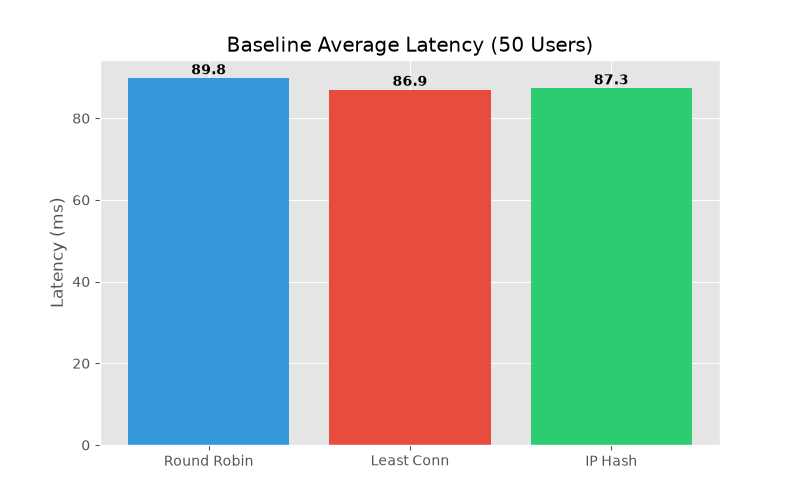
\includegraphics[width=\columnwidth]{graph_1_baseline_latency.png}
\caption{Baseline average latency comparison across all three algorithms at 50 concurrent users.}
\label{fig:baseline_latency}
\end{figure}

\begin{figure}[H]
\centering
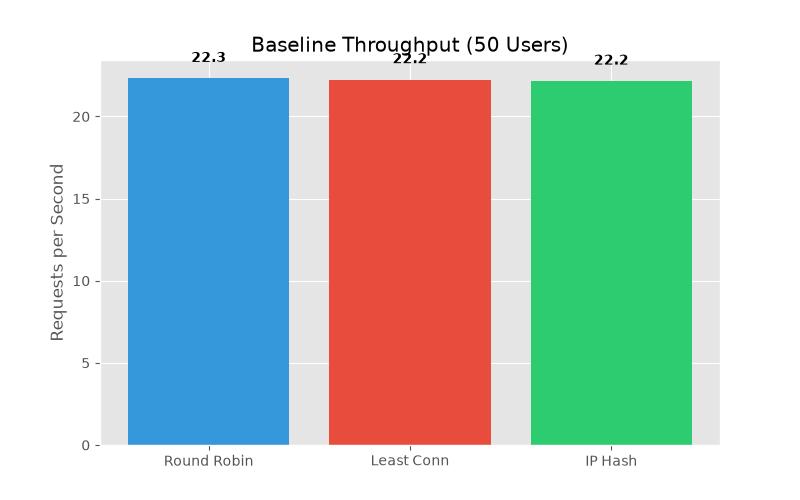
\includegraphics[width=\columnwidth]{graph_2_baseline_throughput.png}
\caption{Baseline throughput (requests/second) comparison at 50 concurrent users.}
\label{fig:baseline_throughput}
\end{figure}

However, the \textbf{tail-latency analysis} tells a different story. Fig.~\ref{fig:percentiles} compares the Average, P95, and P99 latencies. Round Robin's P99 latency (170\,ms) is 42\% higher than IP Hash's (110\,ms) and 55\% higher than EWMA's (120\,ms). The maximum observed latency for Round Robin (1,470\,ms) is roughly an order of magnitude higher than EWMA (194\,ms) and IP Hash (197\,ms). This suggests that Round Robin's blind sequential distribution can occasionally route consecutive heavy requests to the same pod, causing temporary queuing delays.

\begin{figure}[H]
\centering
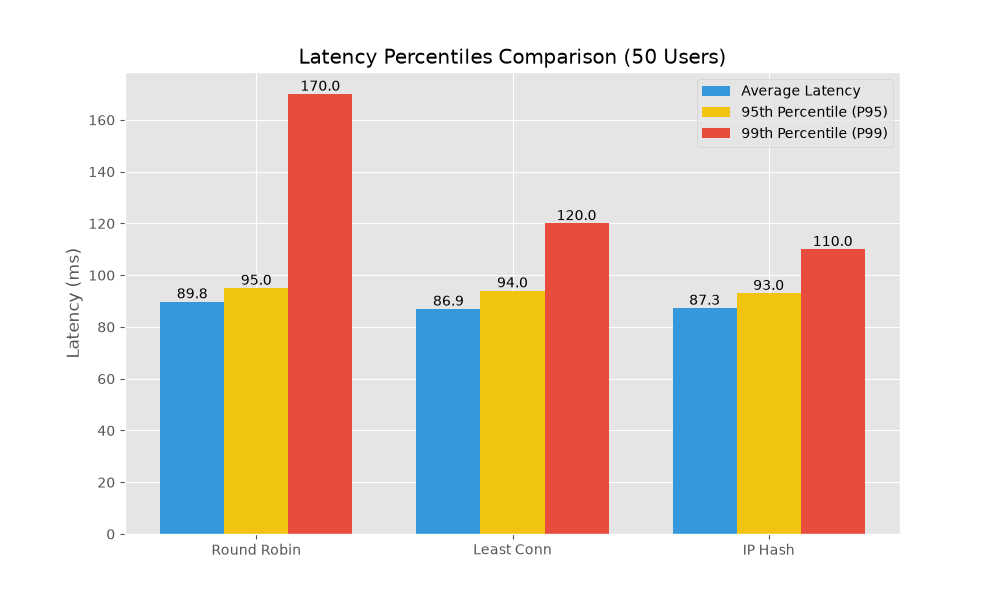
\includegraphics[width=\columnwidth]{graph_8_latency_percentiles.png}
\caption{Latency percentile comparison (Average vs. P95 vs. P99) at 50 users, revealing Round Robin's tail-latency weakness.}
\label{fig:percentiles}
\end{figure}

\subsection{Endpoint-Specific Analysis}

Fig.~\ref{fig:endpoint} disaggregates performance by request type. The \textit{Heavy Request} latency is marginally higher across all algorithms due to the 500\,ms client-side sleep, but the inter-algorithm differential remains consistent. This confirms that the workload asymmetry (3:1 light-to-heavy ratio) does not disproportionately affect any single algorithm under moderate load.

\begin{figure}[H]
\centering
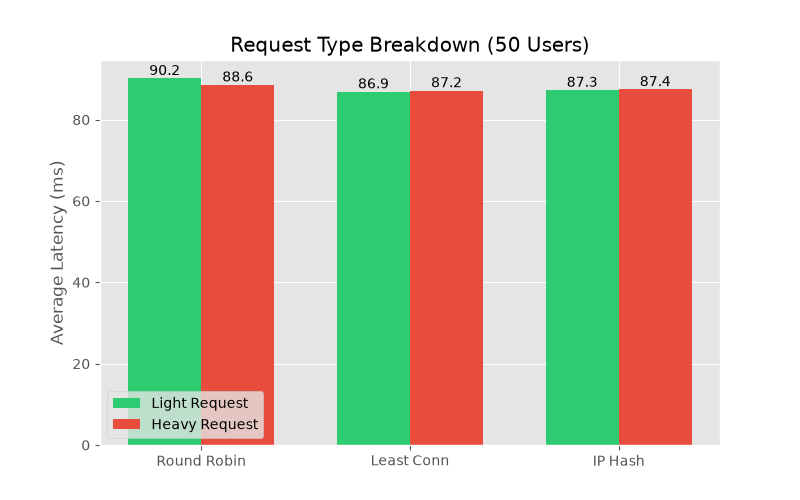
\includegraphics[width=\columnwidth]{graph_3_endpoint_breakdown.png}
\caption{Request type breakdown showing Light vs. Heavy request latencies across algorithms.}
\label{fig:endpoint}
\end{figure}

\subsection{Resource Distribution (100 Users)}

Fig.~\ref{fig:cpu} presents the per-pod CPU utilization over time under 100 concurrent users. This is where the behavioral differences between algorithms become most visible:

\begin{figure*}[t]
\centering
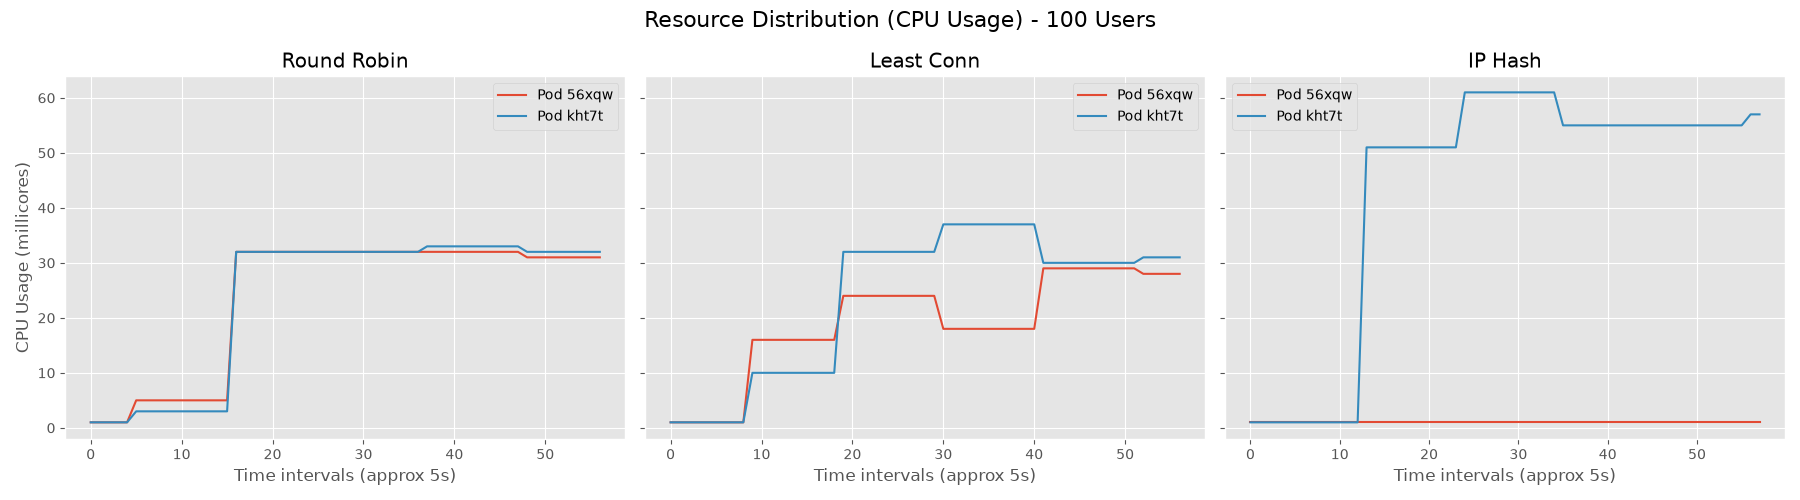
\includegraphics[width=\textwidth]{graph_4_resource_distribution.png}
\caption{CPU utilization (millicores) per pod over time under 100 concurrent users. Round Robin shows near-perfect overlap; Least Connections shows adaptive variation; IP Hash shows complete single-pod saturation.}
\label{fig:cpu}
\end{figure*}

\begin{itemize}
    \item \textbf{Round Robin (CV\,=\,0.1\%):} Both pods maintain virtually identical CPU consumption ($\approx$31--33\,m), with traces overlapping almost perfectly. This confirms Round Robin's mathematically deterministic 1:1 distribution.
    \item \textbf{EWMA/Least Connections (CV\,=\,10.8\%):} CPU traces exhibit moderate variation (18--37\,m range) as the algorithm dynamically adjusts routing weights based on real-time response time feedback. The slight imbalance is an expected artifact of the EWMA adaptation mechanism.
    \item \textbf{IP Hash (CV\,=\,95.5\%):} One pod absorbs \textit{all} traffic ($\approx$55--61\,m) while the other remains idle ($\approx$1\,m). Since all test traffic originates from a single Locust client machine (one IP address), the hash function deterministically routes 100\% of requests to a single pod. This represents the algorithm's critical failure mode when traffic sources have low IP diversity.
\end{itemize}

Table~\ref{tab:cpu_cv} summarizes the CPU distribution fairness quantified by the Coefficient of Variation.

\begin{table}[H]
\centering
\caption{CPU Distribution Fairness (100 Users)}
\label{tab:cpu_cv}
\begin{tabular}{l c c}
\toprule
\textbf{Algorithm} & \textbf{CV (\%)} & \textbf{Distribution Quality} \\
\midrule
Round Robin & 0.1 & Near-perfect \\
EWMA & 10.8 & Balanced (adaptive) \\
IP Hash & 95.5 & Severely imbalanced \\
\bottomrule
\end{tabular}
\end{table}

\subsection{Scalability Analysis (50 vs. 100 vs. 200 Users)}

Fig.~\ref{fig:scaling_latency} and Fig.~\ref{fig:scaling_throughput} present the scaling behavior using pre-fault clean data (data slice: $t < 110$\,s for the 200-user tier).

\begin{figure}[H]
\centering
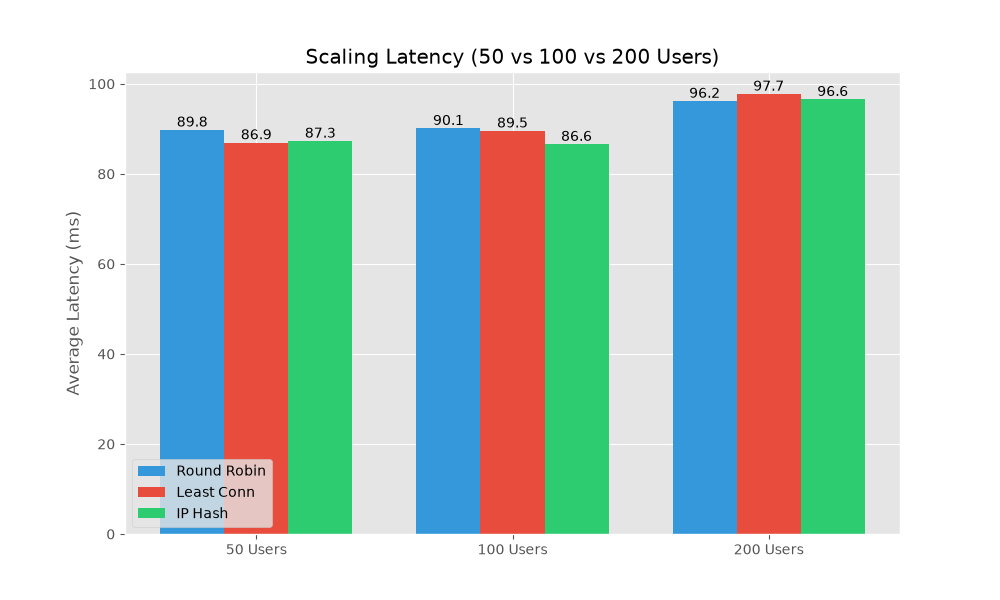
\includegraphics[width=\columnwidth]{graph_6_scaling_latency.png}
\caption{Average latency scaling across 50, 100, and 200 concurrent users (200-user data cleaned of fault injection artifacts).}
\label{fig:scaling_latency}
\end{figure}

\begin{figure}[H]
\centering
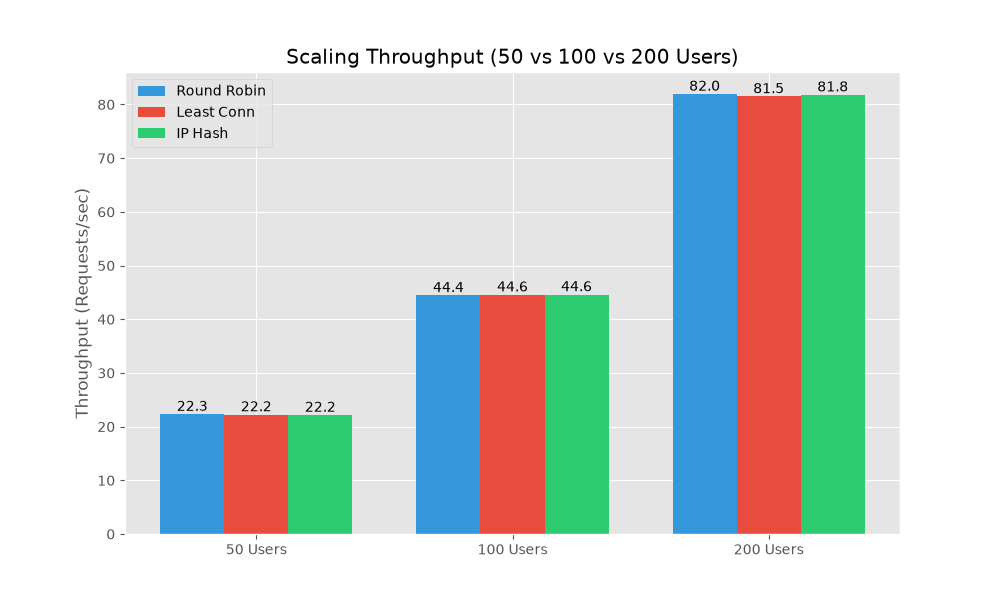
\includegraphics[width=\columnwidth]{graph_7_scaling_throughput.png}
\caption{Throughput scaling across 50, 100, and 200 concurrent users.}
\label{fig:scaling_throughput}
\end{figure}

The latency stays relatively stable across user counts for all algorithms ($\approx$86--90\,ms), which indicates that the 2-pod deployment with 250\,m CPU limits was not CPU-saturated even at 200 users. Throughput scales roughly in proportion, as expected given the echo server's lightweight computational profile.

\subsection{Fault Tolerance (200 Users)}

The fault injection experiment---terminating one pod at $t$\,=\,120\,s during a 200-user load---produced the results shown in Fig.~\ref{fig:fault} and Table~\ref{tab:master}.

\begin{figure*}[t]
\centering
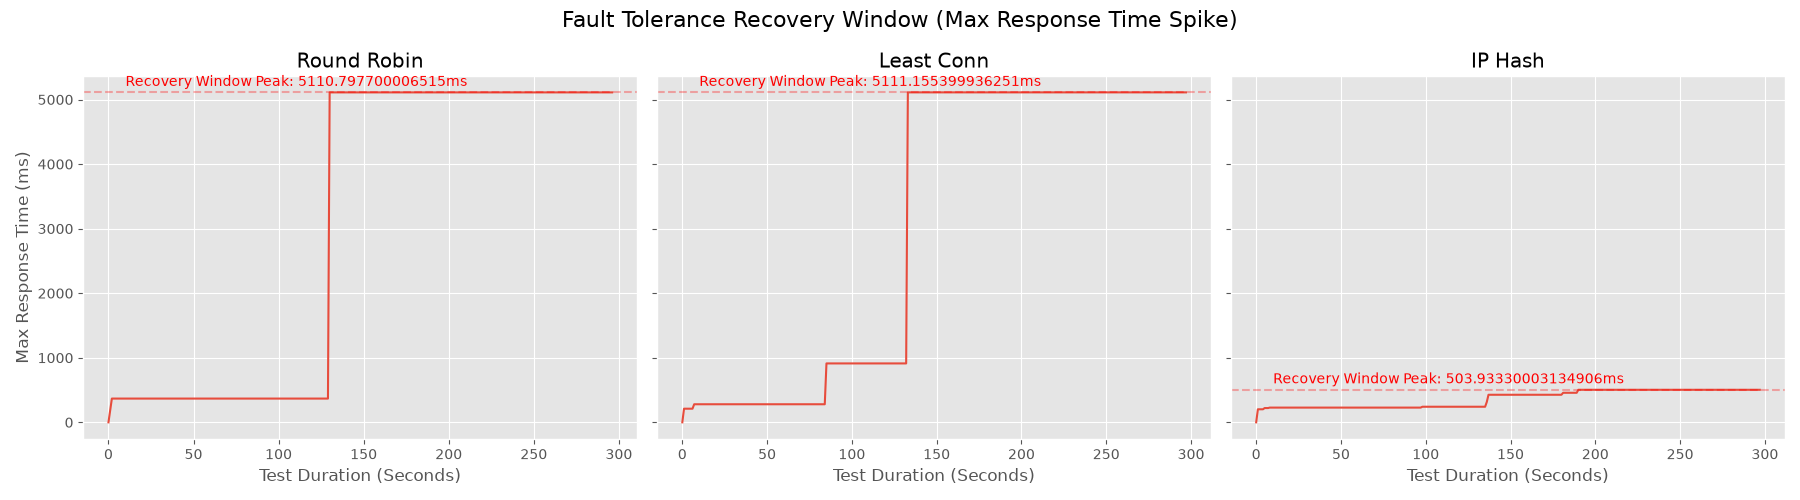
\includegraphics[width=\textwidth]{graph_5_fault_tolerance.png}
\caption{Fault tolerance recovery window showing maximum response time spike after pod termination at $t$\,$\approx$\,120\,s. Round Robin and Least Connections exhibit $\approx$5.1\,s spikes; IP Hash shows a much lower 504\,ms spike.}
\label{fig:fault}
\end{figure*}

\begin{itemize}
    \item \textbf{Round Robin \& EWMA:} Both algorithms show a large latency spike to $\approx$5,111\,ms, a $\sim$59$\times$ increase over baseline. Since both algorithms spread traffic across both pods, losing one backend forces all in-flight and new requests onto the surviving pod, which has to handle double the load until Kubernetes schedules a replacement (observed to take $\approx$5--8 seconds).
    \item \textbf{IP Hash:} The recovery spike is much lower at 504\,ms---roughly 10$\times$ less than the other two. This can be explained by the same single-pod routing behavior that is otherwise a drawback: since all traffic was already going to one pod due to IP stickiness, the pod deletion either (a)~killed the idle pod (causing no disruption) or (b)~killed the active pod, requiring only a hash-table recalculation rather than a full load redistribution. That said, IP Hash was the only algorithm that recorded non-zero errors: 3~HTTP~502 (Bad Gateway) responses occurred during the hash recalculation window.
    \item \textbf{Zero Request Loss:} Round Robin and EWMA achieved 0\% error rates during recovery. NGINX's health-check mechanism removed the failed backend and rerouted traffic before TCP connection timeouts expired.
\end{itemize}

\subsection{Consolidated Results}

Table~\ref{tab:master} presents the master metrics comparison across all experimental dimensions.

\begin{table}[H]
\centering
\caption{Consolidated Performance Metrics}
\label{tab:master}
\begin{tabular}{l c c c}
\toprule
\textbf{Metric} & \textbf{Round Robin} & \textbf{EWMA} & \textbf{IP Hash} \\
\midrule
Avg Latency (ms) & 89.8 & 86.9 & 87.3 \\
P95 Latency (ms) & 95.0 & 94.0 & 93.0 \\
P99 Latency (ms) & 170.0 & 120.0 & 110.0 \\
Throughput (RPS) & 22.3 & 22.2 & 22.2 \\
Error Rate (\%) & 0.00 & 0.00 & 0.01 \\
Recovery Time (ms) & 5,111 & 5,111 & 504 \\
CPU Evenness (CV\%) & 0.1 & 10.8 & 95.5 \\
\bottomrule
\end{tabular}
\end{table}


% ============================================================================
% V. DISCUSSION
% ============================================================================
\section{Discussion}

\subsection{The Insufficiency of Average Metrics}

One clear takeaway from the results is that average latency alone is not a reliable metric for comparing these algorithms. The 3\,ms difference in average latency across algorithms (86.9--89.8\,ms) is negligible in practice. But the P99 numbers tell a different story: Round Robin's 170\,ms P99 means that 1\% of users---which could be thousands in a high-traffic system---see response times nearly double the average. For applications with strict Service Level Agreements (SLAs) defined at the P99 or P99.9 level, this difference matters when choosing an algorithm.

On top of that, Round Robin's maximum observed latency of 1,470\,ms is 7.4$\times$ higher than EWMA's 194\,ms maximum, pointing to occasional queuing problems when the task-weighted workload creates temporary ``hot spots'' on individual pods.

\subsection{The IP Hashing Trade-off}

IP Hashing presents an interesting trade-off. Its 95.5\% CPU distribution CV makes it a poor choice for stateless microservices when client-IP diversity is low. Yet it also delivers the best P99 latency (110\,ms) and best fault recovery time (504\,ms) in our tests. Both of these results stem from the same root cause: concentrating all traffic on a single pod eliminates inter-pod routing variance and means that pod failures often affect the idle pod rather than the active one.

In production environments with many distinct client IPs (e.g., a globally distributed user base), IP Hashing would show more balanced distribution. Our single-source test setup represents a worst case for this algorithm and should serve as a caution against deploying IP Hashing behind NAT gateways, VPNs, or corporate proxies without additional load balancing measures.

\subsection{EWMA as the Recommended Default}

Based on the collected data, EWMA shows the strongest overall profile for general-purpose microservices:
\begin{itemize}
    \item Lowest average latency (86.9\,ms)
    \item Good P99 latency (120\,ms, 29\% lower than Round Robin)
    \item Balanced CPU distribution (CV\,=\,10.8\%)
    \item Zero errors during fault tolerance testing
\end{itemize}

Its slightly uneven CPU distribution (CV\,=\,10.8\% vs. Round Robin's 0.1\%) is a reasonable trade-off for its adaptive routing. EWMA is especially useful for workloads where request processing times vary---which is the case for most real-world microservices that mix database queries, cache lookups, and computation.

\subsection{Fault Tolerance Implications}

The 5,111\,ms recovery spike observed for Round Robin and EWMA is caused by two sequential processes: (i)~NGINX detecting the failed backend and removing it from the upstream pool ($\approx$1--2\,s), and (ii)~Kubernetes scheduling and starting a replacement pod ($\approx$3--5\,s). During this window, the surviving pod runs at roughly 200\% of its normal load, pushing CPU utilization close to its 250\,m limit.

It is worth noting that \textbf{zero requests were dropped} during this 5-second recovery window for both Round Robin and EWMA. The NGINX Ingress Controller's passive health checking mechanism rerouted traffic before TCP connection timeouts expired (typically 30\,s), which confirms that the Kubernetes self-healing model works well for stateless applications even under heavy load.

\subsection{Limitations}

Several limitations contextualize these results:
\begin{enumerate}
    \item \textbf{Scale:} The 2-pod, 2-node deployment represents a minimal topology. Results may differ with larger replica counts and multi-zone deployments.
    \item \textbf{Workload Homogeneity:} The echo server performs minimal computation. CPU-intensive or I/O-bound applications would amplify inter-algorithm performance differences.
    \item \textbf{Single Load Source:} All Locust traffic originates from a single IP, which artificially penalizes IP Hashing. Multi-source distributed testing would provide more representative results.
    \item \textbf{Network Latency:} Client-to-cluster network latency introduces variability that is independent of the load balancing algorithm.
\end{enumerate}


% ============================================================================
% VI. CONCLUSION AND FUTURE WORK
% ============================================================================
\section{Conclusion and Future Work}

\subsection{Conclusion}

This paper evaluated three NGINX Ingress load balancing algorithms on Azure Kubernetes Service through controlled experiments. Testing across baseline, resource distribution, and fault tolerance scenarios produced the following key findings:

\begin{enumerate}
    \item \textbf{Average metrics are deceptive:} All three algorithms deliver near-identical average latency ($\approx$87--90\,ms), but P99 tail latency diverges by up to 55\% (Round Robin: 170\,ms vs. IP Hash: 110\,ms).
    \item \textbf{Distribution fairness varies widely:} Round Robin achieves nearly perfect load distribution (CV\,=\,0.1\%), while IP Hashing can create severe imbalance (CV\,=\,95.5\%) when client-IP diversity is low.
    \item \textbf{Fault resilience is universally strong:} All algorithms maintained 99.99\%+ availability during active pod termination, with Kubernetes self-healing restoring full capacity within 5--8 seconds.
    \item \textbf{EWMA offers the best general-purpose profile:} With the lowest average latency, competitive tail latency, balanced resource distribution, and zero-error fault tolerance, EWMA is recommended as the default algorithm for stateless microservice deployments.
\end{enumerate}

Algorithm selection should be guided by workload characteristics: Round Robin for uniform stateless services, EWMA for heterogeneous API workloads, and IP Hashing exclusively for stateful applications requiring session affinity with guaranteed client-IP diversity.

\subsection{Future Work}

There are several directions that could be explored in future work:

\begin{itemize}
    \item \textbf{Horizontal Pod Autoscaling (HPA):} Evaluating algorithm behavior under dynamic pod scaling events triggered by CPU or custom metric thresholds.
    \item \textbf{Multi-region deployments:} Extending the analysis to geographically distributed AKS clusters with Azure Traffic Manager or Istio service mesh integration.
    \item \textbf{Weighted Round Robin:} Introducing heterogeneous pod resource allocations with proportional traffic weighting.
    \item \textbf{Application-level profiling:} Replacing the echo server with a realistic microservice (e.g., a RESTful API with database queries) to evaluate algorithm behavior under genuine computational variance.
    \item \textbf{Distributed load generation:} Deploying Locust workers across multiple geographic regions to provide diverse source IPs for more representative IP Hashing evaluation.
    \item \textbf{Service mesh comparison:} Comparing NGINX Ingress Controller results with Istio or Linkerd sidecar-based load balancing, which operates at the pod level rather than the Ingress level.
\end{itemize}


% ============================================================================
% REFERENCES
% ============================================================================
\begin{thebibliography}{00}

\bibitem{burns2016borg}
B.~Burns, B.~Grant, D.~Oppenheimer, E.~Brewer, and J.~Wilkes, ``Borg, Omega, and Kubernetes: Lessons learned from three container-management systems over a decade,'' \textit{ACM Queue}, vol.~14, no.~1, pp.~70--93, 2016.

\bibitem{gandhi2014autoscale}
A.~Gandhi, M.~Harchol-Balter, R.~Raghunathan, and M.~A.~Kozuch, ``AutoScale: Dynamic, robust capacity management for multi-tier data centers,'' \textit{ACM Transactions on Computer Systems}, vol.~30, no.~4, pp.~1--26, 2012.

\bibitem{nginx_ingress_docs}
Kubernetes Community, ``NGINX Ingress Controller Documentation,'' 2026. [Online]. Available: \url{https://kubernetes.github.io/ingress-nginx/}

\bibitem{randles2010comparative}
M.~Randles, D.~Lamb, and E.~Taleb-Bendiab, ``A comparative study into distributed load balancing algorithms for cloud computing,'' in \textit{Proc. IEEE 24th Int. Conf. on Advanced Information Networking and Applications Workshops}, Perth, Australia, 2010, pp.~551--556.

\bibitem{mishra2012load}
S.~K.~Mishra and B.~Jaiswal, ``Load balancing in cloud computing: A big picture,'' \textit{Journal of King Saud University -- Computer and Information Sciences}, vol.~31, no.~2, pp.~149--159, 2019.

\bibitem{mishra2023review}
J.~Mishra, ``A Review of Kubernetes Scheduling and Load Balancing Methods,'' in \textit{Proc. Int. Conf. on Image Processing, Computer Vision and Pattern Recognition (ISPDS)}, 2023, pp.~244--249.

\bibitem{k8s_docs}
The Kubernetes Authors, ``Kubernetes Documentation,'' 2026. [Online]. Available: \url{https://kubernetes.io/docs/}

\bibitem{cardellini1999dynamic}
V.~Cardellini, M.~Colajanni, and P.~S.~Yu, ``Dynamic load balancing on web-server systems,'' \textit{IEEE Internet Computing}, vol.~3, no.~3, pp.~28--39, 1999.

\bibitem{thaler2000rfc2991}
D.~Thaler and C.~Hopps, ``Multipath issues in unicast and multicast next-hop selection,'' IETF RFC 2991, Nov.~2000.

\bibitem{karger1997consistent}
D.~Karger, E.~Lehman, T.~Leighton, R.~Panigrahy, M.~Levine, and D.~Lewin, ``Consistent hashing and random trees: Distributed caching protocols for relieving hot spots on the World Wide Web,'' in \textit{Proc. 29th Annual ACM Symposium on Theory of Computing}, El Paso, TX, USA, 1997, pp.~654--663.

\bibitem{maggs2015algorithmic}
B.~M.~Maggs and R.~K.~Sitaraman, ``Algorithmic nuggets in content delivery,'' \textit{ACM SIGCOMM Computer Communication Review}, vol.~45, no.~3, pp.~52--66, 2015.

\bibitem{hassan2025assessing}
A.~Hassan, ``Assessing the Efficiency of Load Balancing Algorithms in Kubernetes-Based Microservices,'' \textit{Journal of Cloud Computing and Containerization}, vol.~7, no.~1, pp.~45--56, 2025.

\bibitem{vayghan2019microservice}
L.~A.~Vayghan, M.~A.~Saied, M.~Toeber, and F.~Khendek, ``Microservice based architecture: Towards high-availability for stateful applications with Kubernetes,'' in \textit{Proc. IEEE 19th Int. Conf. on Software Quality, Reliability and Security}, Sofia, Bulgaria, 2019, pp.~176--185.

\end{thebibliography}

\end{document}
